\documentclass[11pt, twocolumn]{article}
\usepackage{fullpage}
\usepackage{morefloats}
\usepackage{url}
\usepackage{graphicx}
\usepackage{pdftexcmds}
\usepackage{listings}
\begin{document}

\title{Patent Database Search Tool}
\author{Aditya Kaulagi, Gabe Fierro\\
	Coleman Fung Institute for Engineering Leadership\\
	UC Berkeley\\
	\texttt{aditya15@berkeley.edu, fierro@eecs.berkeley.edu}}
\date{\today}
\maketitle

\begin{abstract}
In this document, I describe the process of constructing SQL Queries from a HTML form, which are used to get results from a database. These results are then emailed to the person who requested them.
\end{abstract}

\section{Introduction}
Patent data plays an invaluable role in research into economic trends,
invention, innovation policy and technology strategy. Since the digitization
of patent data starting in 1975, though patent data has been freely
available through the United States Patent and Trademark Office, it
has been difficult to use. We present a substantial improvement in
data quality and accessibility over previous third-party re-releases
of US patent data. This will not only facilitate further research
on up-to-date patent records, but also increase the reproducibility
of previous research results. 

\section{Structure of the Application}
\begin{figure*}
\center
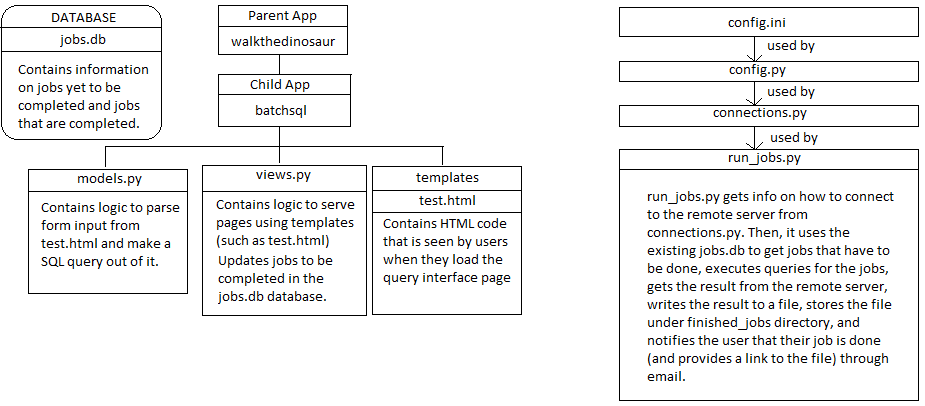
\includegraphics[width=.8\textwidth]{figs/structure}
\caption{Structure of app}
\label{fig:structure}
\end{figure*}

The application is available on github at \verb`https://github.com/gtfierro/walkthedinosaur`. The application consists of three services: the django app that parses user input and turns it into a query, a python file that executes the query, gets the result from the remote MySQL database, writes it to a file and emails the user a notification which contains a download link to the file, and a fileserver that serves files to the user. 

All the models, templates and views are stored in the batchsql folter. The python file that executes the query is called \verb`run_jobs.py`. The information to connect to the remote server and other configurations are stored in \verb`config.ini`.
\section{Structure of Database}
The database$^{[1]}$ is divided into many tables. Out of these tables, the tables we can currently get information from (and their columns) are:

\begin{enumerate}

\item \verb`patent`: This table contains primary information about the patent. 
\begin{enumerate} 
\item title: The Title of the Patent
\item id: The patent ID. This is a unique number for each patent.
\item date: The date on which this patent was issued. 
\item country: The country where this patent was issued.
\end{enumerate}

\item \verb`rawinventor`: This table contains information about the patent’s inventor.
\begin{enumerate}
\item name\_first: The first name of the inventor.
\item name\_last: The last name of the inventor.
\item nationality: The nationality of the inventor.
\item location\_id: Column to establish a relationship between inventors and locations. This contains the id of the location of the inventor.
\item patent\_id: Column to establish a relationship between a patent and its inventor. This contains the id of the patent to which it refers to.
\end{enumerate}

\item \verb`rawassignee`: This table contains information about the entity that assigned this patent.
\begin{enumerate}
\item name\_first: The first name of the assignee.
\item name\_last: The last name of the assignee.
\item nationality: The nationality of the assignee.
organization: Name of the organization this assignee belongs to (if any).
\item location\_id: Column to establish a relationship between inventors and locations. This contains the id of the location of the assignee.
\item patent\_id: Column to establish a relationship between a patent and its assignee. This contains the id of the patent to which it refers to.
\end{enumerate}

\item \verb`rawlawyer`: 
\begin{enumerate}
\item name\_first: The first name of the inventor.
\item name\_last: The last name of the inventor.
\item organization: Name of the organization this assignee belongs to (if any).
\item country: Country where the lawyer (organization) exists.
\item patent\_id: Column to establish a relationship between a patent and its lawyer. This contains the id of the patent to which it refers to.
\end{enumerate}

\item \verb`rawlocation`: This table stores information for different locations.
\begin{enumerate}
\item id: Unique number for each location.
\item city: The name of the city.
\item state: The name of the state.
\item country: The name of the country.
\end{enumerate}

\item \verb`claim`: This table stores information about the claims of every patent.
\begin{enumerate}
\item patent\_id: Column to establish a relationship between a patent and its lawyer. This contains the id of the patent to which the claim refers to.
\item text: The text of this claim.
\item dependent: ID of the claim this claim is dependent on.
\item sequence: ID of this claim.
\end{enumerate}

\item \verb`uspatentcitation`: This table stores information on all the citations in a patent.
\begin{enumerate}
\item patent\_id: Column to establish a relationship between a patent and its lawyer. This contains the id of the patent to which it refers to.
\item date: The date this citation was made.
\item country: The country in which this citation was made.
\item sequence: The ID of the citation.
\end{enumerate}


\end{enumerate}
\section{Converting HTML form to SQL Query}
All of the conversion from HTML form to a SQL query is done in \verb`batchsql/models.py`. All of the form variables are given to the TestQuery class through the post variable that we get from django. In post, all the values entered by the user are stored as a dictionary in the form {“field-name”:”value”}. All form elements are broadly categorized into three types: 

\begin{enumerate}
\item Field Variables: These are the columns that the user wants information from. For example, Name of a Patent, or Name of the Inventor of the Patent.
\item Filter Variables: These are the filters specified by the user. They are mostly textboxes or select lists. If a user enters ‘TX’ under the Inventor’s location filter, then all the rows (in the columns specified by field variables) that have the inventor’s location as ‘TX’ will be returned.
\item Miscellaneous: The csrf token, the email address, the file type that the user wants the information in are considered as miscellaneous fields as models.py does not use these fields to make queries.
\end{enumerate}

	In models.py, we have a dictionary which maps the form elements’ names to (table,column) which they represent. For example, the Patent Title represents the patent table and the title column, and hence one of the entries in this dictionary will be \verb`‘pri-title’:(‘patent’, ‘title’)`(where ‘pri-title’ is the name of the field for Patent Title). All fields have a prefix of ‘f’ to separate them from filters. Converting the form elements is a 4 step process:

\begin{enumerate}
\item Get columns that the users want in their results and store it in a set. This is generated from the Field Variables.
\item Get the names of tables to be searched and store it in a set. This is generated from both the Field Variables and Filter Variables.
\item Get the filter conditions and store it in a set. This is generated from both the Field Variables (for cross-referencing between tables) and Filter Variables.
\item Loop through the above sets and construct a query of the structure\\
\end{enumerate}

\begin{center}
SELECT \{table.columns\} FROM \{tables\} WHERE \{filters\};
\end{center}

	Once this query is generated, it is stored in a local databse that stores the queued and completed job information, and then the \verb`run_jobs.py` file gets this query from this database and runs the jobs that have not yet been completed. It uses sqlalchemy$^{[2]}$ to connect  to and execute queries at the remote MySQL$^{[3]}$ database.
\section{Example Usage}
\subsection{Example 1}
Lets say one needs to get the title of all the patents that had been invented in Texas between the period January 2005 and February 2005. To do this, perform the following steps (screenshots shown after the steps): 

\begin{enumerate}
\item Select the checkbox besides “Title of Patent” in primary information.

\item In the filters section, under Primary information, set From as 2005-1-1 and To as 2005-2-1. Also, type ‘TX’ in inventor’s state textbox. 

\item Finally, type in your email address on the bottom of the page, choose the filetype, and click on “Submit”.
\end{enumerate}

This form is translated into the SQL query:

SELECT patent.title FROM patent, rawinventor, rawlocation WHERE (patent.date BETWEEN ‘2005-1-1’ AND ‘2005-2-1’) AND (patent.id = rawinventor.patent\_id) AND ((rawlocation.state LIKE ‘\%TX\%’) AND rawlocation.id = rawinventor.rawlocation\_id);

\begin{figure*}
\center
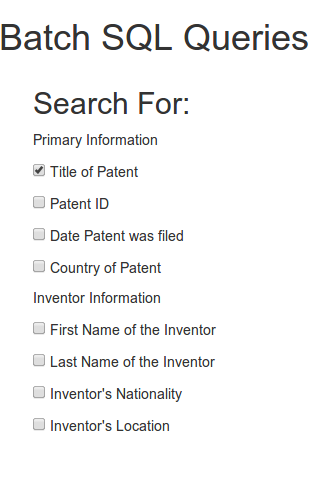
\includegraphics[width=.8\textwidth]{figs/ex1s1}
\caption{Example 1: Step 1}
\label{fig:Step 1}
\end{figure*}

\begin{figure*}
\center
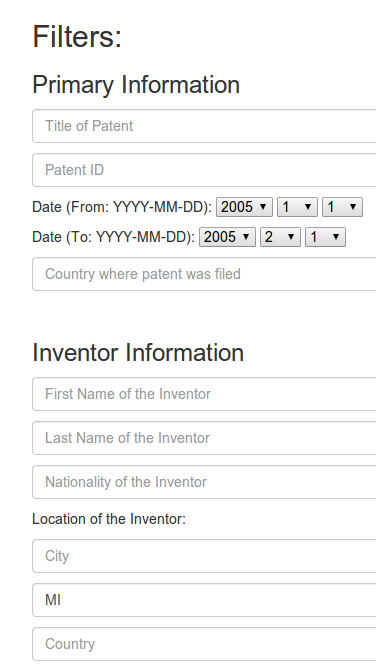
\includegraphics[width=.8\textwidth]{figs/ex1s2}
\caption{Example 1: Step 2}
\label{fig:Step 2}
\end{figure*}

\begin{figure*}
\center
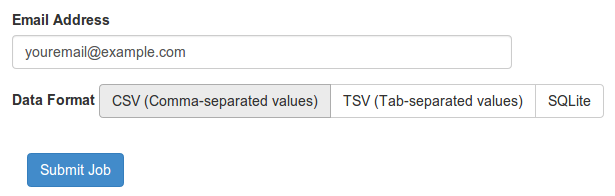
\includegraphics[width=.8\textwidth]{figs/ex1s3}
\caption{Example 1: Step 3}
\label{fig:Step 3}
\end{figure*}


\subsection{Example 2}
For the second example, lets say one needs to get the names (first and last) of the lawyers that filed for a patent in Michigan between January 2005 and February 2005. In addition, say they want the inventors and assignees to also be in Michigan$^{[5]}$.

\begin{enumerate}

\item Select First Name of Lawyer and Last Name of Lawyer under Lawyer Information.

\item In the filters section, make sure to fill in dates as before, and this time, fill in the textbox for Inventors State with ‘MI’ and same for the Assignee’s State textbox.

\item Finally, just as before, fill in your email, choose your filetype, and click on “Submit”.

\end{enumerate}

This form is translated into the SQL query:

SELECT rawlawyer.name\_first, rawlawyer.name\_last FROM patent, rawlocation, rawinventor, rawassignee, rawlawyer WHERE (patent.date BETWEEN ‘2005-1-1’ AND ‘2005-2-1’) AND (patent.id = rawinventor.patent\_id) AND (rawassignee.patent\_id = rawinventor.patent\_id) AND (rawlawyer.patent\_id = rawinventor.patent\_id) AND ((rawlocation.state LIKE ‘\%MI\%’) AND rawlocation.id = rawinventor.rawlocation\_id) AND ((rawlocation.state LIKE ‘\%MI\%’) AND rawlocation.id = rawassignee.rawlocation\_id);

\begin{figure*}
\center
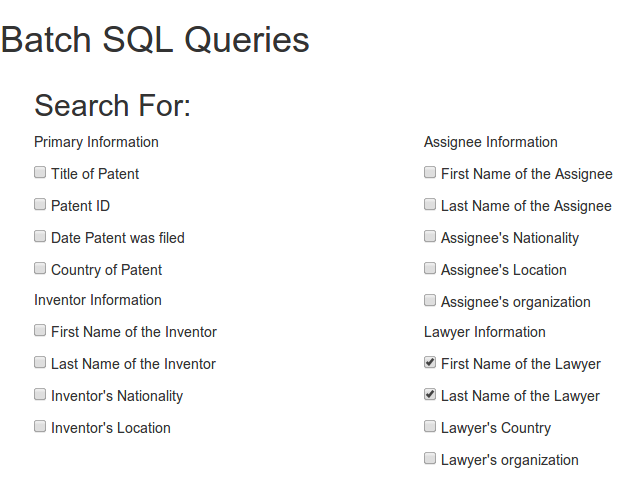
\includegraphics[width=.8\textwidth]{figs/ex2s1}
\caption{Example 2: Step 1}
\label{fig:Step 1}
\end{figure*}

\begin{figure*}
\center
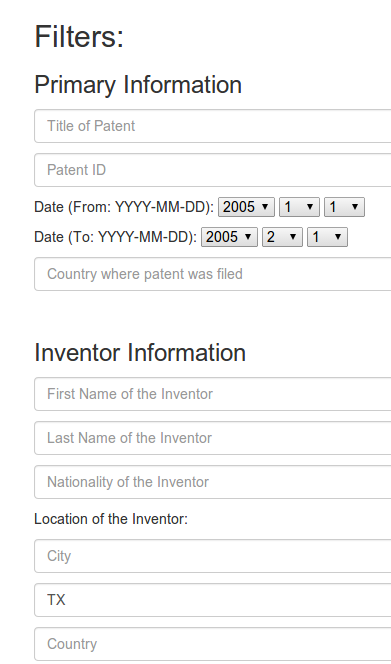
\includegraphics[width=.8\textwidth]{figs/ex2s2-1}
\caption{Example 2: Step 2-1}
\label{fig:Step 2}
\end{figure*}

\begin{figure*}
\center
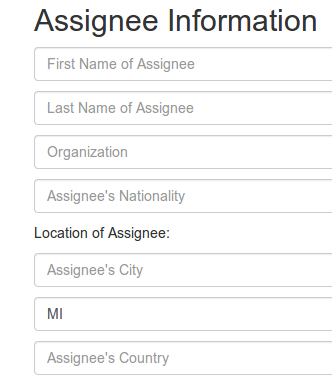
\includegraphics[width=.8\textwidth]{figs/ex2s2-2}
\caption{Example 2: Step 2-2}
\label{fig:Step 3}
\end{figure*}


\section{Acknowledgements}
I would like to thank Professor Lee Fleming for giving me the opportunity to work on this project. I would also like to thank Gabe Fierro for guiding me in making the application and helping me fix many bugs and design issues.

{
\scriptsize
\bibliographystyle{acm}
\bibliography{patentprocessor}
}

\end{document}
